\documentclass[11pt,a4paper]{report}

\usepackage{url}
\usepackage[utf8]{inputenc}
\usepackage{graphicx}
\usepackage[all]{xy}
\usepackage{amsmath}
\usepackage{amsthm}
\usepackage{todonotes}
\usepackage{array}
\usepackage{listings}
\usepackage[a4paper]{geometry}
\usepackage[breaklinks]{hyperref}

\makeatletter %otherwise geometry resets everything
\Gm@restore@org
\makeatother

\setlength{\itemsep}{0cm}
\setlength{\voffset}{0cm}
\setlength{\headheight}{0cm}
\setlength{\topmargin}{0cm}
\setlength{\extrarowheight}{3pt} %for superscripts in tabular
\setlength{\arraycolsep}{4pt}
\lstset{basicstyle = \footnotesize, breaklines = true}

\graphicspath{{imgs/}}
\begin{document}
\begin{titlepage}
    \begin{center}
        \textsc{\LARGE Bachelor thesis\\Computing Science}\\[1.5cm]
        
\includegraphics[height=100pt]{logo}

        \vspace{0.4cm}
        \textsc{\Large Radboud University}\\[1cm]
        \hrule
        \vspace{0.4cm}
        \textbf{\huge DGA-based Malware Detection Using DistilBERT}\\[0.4cm]
        \hrule
        \vspace{2cm}
        \begin{minipage}[t]{0.45\textwidth}
            \begin{flushleft} \large
                \textit{Author:}\\
                Abdulkarim Abdulkadir\\
                s4840933\\
                abdulkarim.abdulkadir@ru.nl
            \end{flushleft}
        \end{minipage}
        \begin{minipage}[t]{0.45\textwidth}
            \begin{flushright} \large
                \textit{First supervisor:}\\
                Assistant Professor Katharina Kohls\\
                \texttt{kkohls@cs.ru.nl}\\[1.3cm]
                \textit{[Second supervisor:]}\\
                title, name\\
                \texttt{e-mail adress}\\[1.3cm]
                \textit{Second assessor:}\\
                title, name\\
                \texttt{e-mail adress}
            \end{flushright}
        \end{minipage}
        \vfill
        {\large \today}
    \end{center}
\end{titlepage}

\begin{abstract}
    Malware use domain generation algorithms (DGAs) to generate pseudo-random domain names to evade supervision. In order to defend against DGA traffic, security researches have to discover and comprehend the algorithm by reverse engineering malware samples and register these domains in a DNS blacklist. Eventhough this list has to be frequently updated, it still is readily circumvented by malware authors. An alternative approach is to detect DGA generation using deep learning techniques to classify domains. Recent work in DGA detection have leveraged deep learning architectures such as convolutional neural netowrks (CNNs) and long shor-tterm memory network (LSTMs) to classify domains. However, these classifiers perform inconsistently. Specifically wordlist-based DGA families have been a struggle for these architectures. We propose a novel model based on a distilled version of Bidirectional Encoder Representation from Transformers (DistilBERT) to detect DGA domains. The word embeddings are pre-trained on a large unrelated curpus to learn contextual embeddings for words bidirectionally. Afterwards, the pre-trained parameters enables for short training durations on DGA domains, while the language knowledge stored in the representations grants high performance with a small training dataset. We show that our model outperforms existing techniques on DGA classification, while less time is needed to train our model. Experiments in this paper are run on open datasets and the models' code is provided to reproduce the results.
\end{abstract}


\tableofcontents

\chapter{Introduction}\label{introduction}

% The introduction of your bachelor thesis introduces the research area, the
% research hypothesis, and the scientific contributions of your work.
% A good narrative structure is the one suggested by Simon Peyton Jones
% \cite{peys04:HowToWriteAGoodResearchPaper}:
% %
% \begin{itemize}
% \item describe the problem / research question
% \item motivate why this problem must be solved
% \item demonstrate that a (new) solution is needed
% \item explain the intuition behind your solution
% \item motivate why / how your solution solves the problem (this is technical)
% \item explain how it compares with related work
% \end{itemize}
% %
% Close the introduction with a paragraph in which the content of the next chapters
% is briefly mentioned (one sentence per chapter).

As the purpose of our digital devices continue to expand, the importance of protecting our sensitive data has become more crucial. The pandemic has proven how much we rely on these devices. The value of our digital resources has increased, which makes this an appealing target for exploitation.\\\\ 
A malicious software, or malware, is a software that target our digital resources. The emerging presence of malware have created different types of malware and new attack methods to our computer systems. According to the AV-Test report, in 2021 the number of malware totaled around 1320 million, a 13 times increase of the report in 2012, which was around 100 million \cite{avtest}.\\\\
Most types of modern malware communicate with external servers of the attackers using different network protocols. DNS (Domain Name Server) is a network protocol used frequently to connect to these externel servers \cite{ist}. The malicious external servers have different domain names to make sure to be available to the malwares. An external server having a single domain or a fixed IP address can be blacklisted. This would make the server not accesible anymore. Therefore, external servers create multiple domain names for the malware to connect to. The multiple domain names are created by generating them using a domain generated algorithm (DGA). The malwares are packed with the same DGA that the external server uses, so that it can generate the same domain names. The domain names generated by the servers are registered in advance to secure those domain names. The malware uses Domain Name Server (DNS) services to connect to each generated domain name till it succesfully conncected to the IP address of the malicious external server.\\\\
\pagebreak
\\\\Recently malware that uses DGA are polymorphic. The malware can generate domain names dynamically. One way to do that is by using time information as a seed for the DGA \cite{arntz_2016}. The polymorphic aspect of the malware improves the concealment and robustness of the malware and brings great challenges to DGA-based malware detection. \\\\ 
Hence, there is a solution needed to defend against DGA-based malware. Traditional detection methods use DNS traffic or domain name language characteristics to extract feature out of the DGA malware. After that machine learning is used to analyze the extracted features and complete the identification and classification of DGA domain names. However, it is difficult to determine the DNS traffic and domain name language characteristics of different types of DGA. Specifically, DGA types that use wordlists to generate domains are difficult to differentiate from benign domains. Therefore, detection schemes based on feature extraction and DNS traffic have a high time and bandwidth cost, and the features that are extracted are not flexible. \\\\ 
More comprehensive tactics are necessary to detect malicious domain names and differentiate them from benign domain names. An improved detection method compared with previous approaches is the detection model based on deep learning. The benefit of deep learning is the automatic extraction of the DGA domain features as well as understanding the context of the domain names.\\\\ We propose a nouveau detection model based on deep learning, the Bidirectional Encoder Representations from Transformers (BERT) to detect DGA domains. BERT is a transformer-based machine learning technique which allows for bidirectional training in models. This in contact to previous efforts, which train on a text sequence from left to right or right to left. The second benefit to BERT is that it is already pretrained on different language representation models \cite{DBLP:journals/corr/abs-1810-04805}. \\\\ 
The original English-language BERT base model is pretrained from unlabeled data from the BooksCorpus \cite{BooksCorpus} with 800M words and English Wikipedia with 2500M words \cite{ColBERT}. In our research we will use a distilled version of BERT, called DistilBERT \cite{Sanh2019DistilBERTAD}. This model recuces the size of BERT by 40\%, while still retaining 97 \% of its language understanding capabilities and being 60\% faster. With our DistilBERT model that is pretrained on uncased English words, we are able to detect DGA domains with low-cost, while still surpassing previous detection models.
\pagebreak
\\\\
The paper is structured as follow. In chapter two we will shortly explain what malware is and what kind of malware types there exist. We will describe how botnets use domain generated algorithms to stay online and avoid detection. After that we will describe machine learning, specifically different neural networks techniques, from older neural network techniques to newer ones. We will discuss what kind of problems and shortcomings these older neural networks have compared to the newer ones. Lastly we will introduce a new deep learning model, called the transformer model. As well as unfold the BERT and DistilBERT models that are transformer-based. We will clarify the benefits of these transformer-based models and how it solved several problems of the older neural network techniques. \\\\
In chapter three we will show a detailed implementation of our DistilBERT detection model to detect DGA-based malware domains. Thereafter, show the kind of results our DistilBERT model has produced. Finally, we will compare our results with previous results of DGA detection models.\\\\
In chapter four we will examine previous research done in DGA detection, while looking at their results and their shortcomings.\\\\
In chapter five we will evaluate all our results and discuss the problems our model has and how to improve it. We will conclude by giving any suggestions for future research in this field.
\chapter{Preliminaries}\label{preliminaries}
% This \emph{optional} chapter contains the stuff that your reader needs to know
% in order to understand your work.  Your ``audience" consists of fellow third
% year computing science bachelor students who have done the same core courses
% as you have, but not necessarily the same specialization, minor, or free
% electives.
This section will describe malware, the different types and how it utilizes DGA
perform malicious act. It will also explain the basics of Machine Learning and the types of Neural Networks that are necessary for this research paper to comprehend. \\\\ 
Malware is a blending of two words, malicious and
software, where it clearly defines the functionality of it, namely a software
that is malicious in nature. Malware can have multiple purposes. Cybercriminals
typically use it to extract data from the victims computer to leverage against
them for financial gain. This data can range from financial data, sensitive
personal data: such as healthcare records, personal emails, passwords, etc. The
possibilities of the information that can be compromised are endless.\\\\ The
most common ways victims receive malware is through the internet and mail.
Malware can penetrate a victim's computer in different ways, such as: surfing to
hacked websites, viewing malicious ads on websites, download infected files and
install malicious programs or apps. When a malware has infected the computer
system of a victim, it can come in many forms, such as Ransomware, Spyware,
Trojans, Worms, etc.
\section{Botnets}
A compromised machine that is infected
by malware can end up a network of infected machines (botnets). This machine is
a bot in that network that receives and responds to commands from the command \&
control server. The C \& C server is controlled by and receives commands by a
human controller called a botmaster. The botmaster conceals itself by employing
a number of proxy machines, called the stepping stones, between it and the C \&
C server.  
\pagebreak 
The life cycle of a botnet can be divided into four
phases. For this research only the first two phases are important. The first
phase is when the machine (bot) receives the malware and executes the binary.
After the machine is infected, this machine (bot) tries to contact the C \& C
server to announce its presence and contact with it. This establishment phase is
called Rallying. There are two ways that the bot can contact with the C \& C
server. The first way that the bot knows the IP address of the C \& C server.
This IP address can be hardcoded into the binary, which can be exposed 
by reverse engineering the binary. The IP address can also be seeded,
where the bot is provided by a list of peers, this list can be hidden in Windows
registries.  The second way is that the bot knows the domain name of the C \& C
server.  The domain name can be hardcoded into the bot binary, where it can
resolve to different IP addresses.  Reverse engineering this binary may expose
the domain name, which can then be blacklisted.
\section{Domain Generated Algorithm}
The domain name can also be generated, then the bot dynamically contacts the C \& C server using DGA (Domain name Generation Algorithm).  The essence of this algorithm is that it creates a set of random strings. The bot attempts to resolve the generated domain names by sending DNS queries until one of the domains resolves to the C \& C server IP Address. The domains that do not resolve will result in Non-Existent Domain (NXDomain) responses.\\\\ The domain names that are generated by the DGA are also known as Algorithmically Generated Domains (AGD).  The DGA uses a seed to serve as a shared secret between the botmaster and the bot. There are two types of seeds: static seed and dynamic seed. The seed is required to calculate the AGDs. The DGA takes the seed value as input to generate pseudo-random strings and append algorithmically TLD (Top Level domains) such as \textit{.nl, .com, .org, .edu}. The static seed can be dictionary of words, random strings that are concatenated, numbers or any other value that the botmaster can come up with. Dynamic seeds are dynamic, it changes with time. Dynamic seeds can be currency exchange rate, daily trending twitter hashtag, weather temperature and current date and time.  The static and dynamic seed elements are then stitched together to generate a pseudo-random string.\\\\ The botmaster uses the DGA to generate a large number of domain names for the C \& C server.  The constant change of domain names for the C \& C server using DGA is known as Domain-Fluxing.  The botmaster registers one of the DGA created domain names for the C \& C server in advance using the same algorithm of the DGA.  When the bot receives the malware, the malware queries to the pre-registered domain name and resolves the IP address using DNS.  The botmaster registers the domain name most of the time some hours prior to an attack and disposes of the domain names within a day.  Whenever the previous domain name that the bot connected with does not resolve anymore, it queries to the next set of generated domain names until it find one domain that works.\\\\ The DGA and constant domain-fluxing of the C \& C server provides agility and resilience to the infrastructure of the botmaster.  This makes it hard to predict what domain names a bot will try. Analyst will re-engineer DGA by analyzing the malware and understand how the algorithm works. It is still hard to predict what kind of seed the DGA will use on a specific time. It is also infeasible to report all the domain names that are generated. As some DGA use english dictionary as static seed values, it is hard to distinguish benign domain names from malicious ones.  
\section{Machine Learning}
Machine learning has recently been an attractive tool to be used in security. One way to combat DGA is to use machine learning to find the structure of the generated domains. The machine learning methods can be either supervised or unsupervised. Unsupervised learning uses algorithms to analyze and cluster data, in this case the domains. These algorithms discover hidden patterns or data groupings, without a need for a human intervention. There are three ways to approach unsupervised learning: clustering, association and dimensionality reduction. The domains are divided into clusters to find statistical attributes for each group. To produce a cluster with good generalization capabilities, it can take a lot of time and  effort \cite{unsupervised}. Supervised learning does not rely on the statistical attributes  for each group to find DGAs. Supervised learning attempts to understand and classify the input and predict the outcome accurately. The relationship is represented as a structure to predict the outputs for some specific future inputs.  
\subsection{Neural Networks}
Artificial Neural Networks are artificial systems that were inspired by the biological counterpart. The systems learn in a supervised manner to perform tasks by using various datasets and examples. These neural networks are composed of node layers, containing one or more input layers, hidden layers and output layers. Each node is connected to another node and has an associated weight w and threshold. When the threshold of a specific node is above a certain threshold value, then that node is activated, otherwise no data is passed along to the next layer of the network. \\\\ 
The network uses training data to learn and improve the accuracy of the network. This is usually done by backpropagation. Backpropagation is a supervised learning algorithm that computes the difference between the model output and the actual output using gradient descent\cite{gradient_descent}. It checks if the error is minimized and update the weights and biases accordingly. It repeats the process until the error becomes minimum.  

\subsection{Activation Functions}
The activation functions in a neural network are functions that de

\subsection{Recurrent Neural Networks}
Recurrent neural networks are a type of neural network that uses the output from the previous step and fed that as input in the current step, while in traditional Neural networks the network assumes that the inputs and outputs are independent of each other. It is known for its feedback loops. Recurrent Neural Networks are used for Sequence Modeling. Sequence Modeling is the task to predict about future outcomes. 


\subsection{Vanishing Gradient problem}
\subsection{LTSM}
\subsection{The core of LTSM}
\subsection{Transformers}
\chapter{Research}\label{research}
% This chapter, or series of chapters, delves into all technical details that are
% required to \emph{prove} your scientific hypothesis.
% It should be sufficiently detailed and precise in order for any fellow computing scientist student to be able to \emph{repeat}
% your research and therewith establish the same results / conclusions that you have obtained.
% Please note that, in order to improve readability of your thesis, you can put a part of this information also in one or
% more appendices (see Appendix \ref{appendix}).

In this section we will explain the technical details of our DistilBERT model. First, we will justify which libraries and framework we used for our model. Second, we will showcase how we have implemented the libraries in python to create our model. Afterwards, we will analyze our dataset, consisting of malicious and benign domains. Lastly, we will demonstrate the results of our model. The python notebook code is accessible in \ref{appendix}.

\section{System Architecture}
To build and train our DistilBERT model, we used the ktrain library \cite{maiya2020ktrain}. Ktrain is a lightweight open source wrapper for the deep learning library TensorFlow Keras \cite{chollet2015keras}. According to the authors, it helps to build, train and deploy neural networks in a more accessible and easier way. Ktrain allows you to easily estimate an optimal learning rate for your model given a learning rate finder.\\\\
For data analysis on our dataset, we use the open source scikit-learn library \cite{sklearn_api}. It is a simple and efficient tool to predict and analyze data, built on NumPy, SciPy and matplotlib.


\section{Datasets}
This paper uses two open datasets to make the research reproducible. The Tranco one million domains \cite{Tranco} are used for benign, non DGA, domains. Tranco is a research-oriented top sites ranking dataset that is hardened against manipulation. Most researchers \cite{Antonakakis}\cite{Lison}\cite{Highnam}\cite{TRAN20182401} rely on popularity rankings such as the Alexa top one million domain list. However, the Tranco paper \cite{Tranco} finds out that it is trivial for an adversary to manipulate the composition of these lists. The list of Alexa top one million can be altered by as little as a single HTTP request by adversaries. 
\\
Therefore, the Tranco paper comes up with an one million domain list that is hardened against these manipulations. This is the list we use for our DGA domain detector. We only use a fourth of the domains in the 1 million Tranco list, totalling $200000$ benign domains.\\\\
For the DGA malicious domains, we use the UMUDGA dataset \cite{UMUDGA}. UMUDGA is a dataset for profiling DGA-based botnets. It contains 37 notorious distinct malware variants generated domain lists. For our model, we have opted out for approximately $5000$ domain lists per malware variant. Our DGA domains totals $184765$. Combined we have a total of $384765$ domains in our dataset, with a proportion of 52\% between benign and DGA domains.

\section{DistilBERT Detector}
To prepare our dataset for the detector, we first separate our dataset into input (X) and output (y) columns.  Then, we use the sklearn library function \textit{train\_test\_split(X,y, test\_size, random\_state)}, which splits our dataset into a random train and test (validation) dataset. This function uses a random state, which accepts an integer seed to control the shuffling applied to the data before the split. The test\_size indicates the percent of the dataset that will be allocated to the test set. For our model, the proportion between train and test date is 25\% and 75\% respectively.\\\\
The ktrain library wraps pre-trained, fast and easy to use models that can be applied to our text data. The text classification model that we will use for our detector is the DistilBERT \cite{Sanh2019DistilBERTAD} model. As mentioned in the introduction, it is a distilled version of BERT, that reduces BERT by 40\%, while still retaining 97\% of its language understanding capabilities and being 60\% faster. DistilBERT is pre-trained on the same data as BERT \cite{ColBERT}. In our model we use the English uncased base pre-trained DistilBERT model. The texts in the model are lowercase and tokenized using WordPiece \cite{WordPiece} and a vocabulary size of $30000$. The DistilBERT model is trained on 8, 16 GB V100 for 90 hours. We use this model to preprocess our training and test data using the ktrain wrapper. 


\subsection{Learning Rate}
We wrap our preprocessed training and test dataset into the \textit{ktrain.Learner} object using the \textit{ktrain.get\_learner(model, train\_data, val\_data, batch\_size)} function. We use a batch size of six for our network. The batch size is the number of samples that will be passed through to the neural network.\\\\
\\The important hyperparameters that we have to set for our neural network is the learning rate. To properly train a neural network, we have to minimize the loss function. If the learning rate is too high, training will not be minimized. However, if the learning rate is too low, training will be slow or can stall. 
To have an optimal learning rate for our model, we can simulate the training by starting with a low training rate and gradually increasing it. As written by Leslie Smith \cite{Learning_Rate} in his paper, he indicates that when plotting the learning rate versus the loss, a good choice for training is the maximal learning rate associated with a still falling loss. This is referred to by Smith as an LR Range Test, or as an LR Finder. The LR Finder can be executed in ktrain as well using the function \textit{lr\_find()} and produce a plot with the \textit{lr\_plot()} function. We can select the maximal learning rate where the loss is still falling prior to divergence in the plot.\\\\ 
A number of studies have shown that by varying the learning rate during training can improve performance to a neural model in terms of both loss minimization and better validation accuracy. A learning rate schedule, such as the 1cycle learning rate schedule \cite{cycle_learning_rate} has benefits to the learning rate. Ktrain has a \textit{fit\_onecycle} function that employs the 1cycle policy. This policy increases for the first half of the training the learning rate from a base rate to a maximum rate, while decays the learning rate to a near-zero value for the second half of the training. Therefore, the maximum learning rate is set using the learning rate finder function mentioned above as well as using the 1cycle learning rate function to train our model.
After we have applied the \textit{lr\_find()} function on our model and plotted this with the \textit{lr\_plot()} function \ref{figure_lr}. We select the maximal learning rate where the loss is still falling prior to divergence. Therefore we choose $3^{e-5}$

\begin{figure}[!htb]
    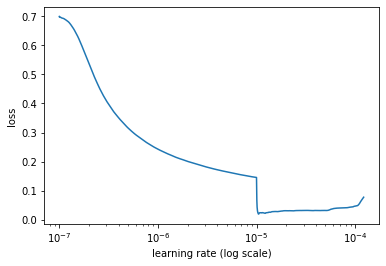
\includegraphics[width=10cm]{DistilBERT_detector_1}
    \caption{DistilBERT LR Range test result}
    \label{figure_lr}
\end{figure}
\pagebreak

\section{Metrics For Validation}
To measure our model performance, we calculate multiple metrics that are used commonly in machine learning research. To illustrate the metrics, we will use the following abbreviations: true positive (TP), true negative (TN), false positive (FP), false negative (FN), true positive rate (TPR) and false positive rate (FPR). The metrics are calculated as follows:

$${
            Precision = \frac{\sum TP}{\sum TP + \sum FP}
        }
$$

The precision metrics measures the ratio of correct positively labeled instances to all positively labeled instances.

$${
            Recall = \frac{\sum TP}{\sum TP + \sum FN}
        }
$$

The recall metrics measures the ratio of correct positively labeled instances to all instances that should have been labeled positive.

$${
            F_1 = 2 \cdot \frac{Precision \cdot Recall}{Precision + Recall}
        }
$$

$F_1$ is the harmonic mean of Precision and Recall.
\pagebreak
$${
            TPR = \frac{\sum TP}{\sum TP + \sum FN}
        }
$$
\\True Positive Rate (TPR) is a synonym for Recall.

$${
            FPR = \frac{\sum FP}{\sum FP + \sum TN}
        }
$$
False Positive Rate (FPR) determines the rate of incorrectly identified labeled instances.
$${
            Accuracy = \frac{TP + TN}{TP + TN + FP + FN}
        }
$$
Accuracy is the fraction of predictions our model solved correctly.
\\\\
The receiving operating characteristics (ROC) curve is an evaluation metric for binary classification problems that plots TPR and FPR at various threshold values. It essentially separates the 'signal' from 'noise'. The ROC curve is a good metric to find out if our neural network is overfitting. The area under the curve (AUC) is an area under the ROC curve that compares ROC curves. Models whose predictions are 100\% wrong, have an AUC of 0.0, whereas models whose predictions are 100\% correct have an AUC of 1.0.

\section{Experiment}

This section evaluates the performance of our DistilBERT model. All operations are performed on a Google Cloud platform. We utilized the Google Colab Pro+ features, which gave us access to 1 V100 GPU, 53 GB of RAM and 8 CPU cores.\\\\ 
We have trained our model for 8 hours, 33 minutes and 13 seconds in 4 epochs. It had an accuracy of $0.9877$ for the train data and $0.9809$ for the test (validation) data. In figure \ref{figure_model} we can find our learner performance in each epoch on our train and validation data.
\begin{figure}[!htb]
    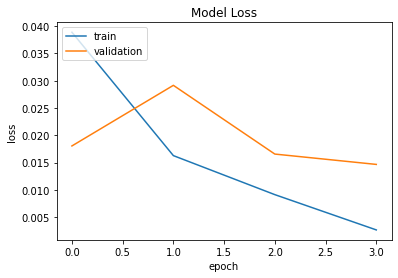
\includegraphics[width=10cm]{DistilBERT_detector_2}
    \caption{Calculating our training performance: loss of our model in each epoch for our train and validation dataset}
    \label{figure_model}
\end{figure}
\pagebreak
\\Whenever the model is trained, we have to cross-check the model with the test data. For that we can use the \textit{validate} function of the ktrain library. The results of our experiments are given in Table \ref{general_results}. We can observe that our model performed exceedingly well, having an accuracy of 99\%. Furthermore, both the benign and DGA domains, totalling $96192$, have an average of 99\%.\\\\
In order to find out how our model performed on each specific DGA family, we evaluated all 37 DGA families and benign domains to get their Precision, Recall and F1-score. The results of that experiment can be found in Table \ref{specific_results}. While evaluating the results, we are able to observe that our model has a better performance on non dictionary-based DGA than dictionary-based DGA families. Dictionary-based DGA families such as \textit{nymaim, matsnu, gozi} have a score lower than the average score of 99\%. A possible reason for this could be that our dataset has more non dictionary-based DGA families compared to dictionary-based DGA families. Our model has more training data on non dictionary-based DGA families, therefore our model is more bias towards them. Our model also seems to struggle more with short-length DGA domains, like \textit{proslikefan, pykspa} DGA families, that have a shorter domain name (URL) compared to other DGA families. This could be, because our DistilBERT model is pre-trained on long English sentences.\\\\  
We also evaluated the ROC-AUC score for our model. Our model has an ROC-AUC score of $0.9997$. This score surpassed the ROC-AUC score of previous research, such as \cite{Highnam} and \cite{Woodbridge}.


\begin{table}[!htb]
    \centering
    \begin{tabular}{llrll}
        \hline
                     & Precision & Recall & F1-score & Support \\ \hline
        benign       & 0.9955    & 0.9964 & 0.9964   & 50103   \\
        DGA          & 0.9961    & 0.9951 & 0.9956   & 46089   \\ \hline
        accuracy     &           &        & 0.9958   & 96192   \\
        macro avg    & 0.9957    & 0.9957 & 0.9957   & 96192   \\
        weighted avg & 0.9958    & 0.9958 & 0.9958   & 96192   \\ \hline
    \end{tabular}
    \caption{Results of our DistilBERT model, expressed in Precision, Recall and F1-score}
    \label{general_results}
\end{table}

\begin{table}[!htb]
    \rowcolors{2}{gray!25}{white}
    \centering
    \scalebox{0.85}{
        \begin{tabular}{l|l|llll}
            \hline
            nr & DGA          & Precision & \multicolumn{1}{r}{Recall} & F1-score        & Support \\ \hline
            1  & alureon      & 1.0000    & 0.9905                     & 0.9952          & 1268    \\
            2  & banjori      & 1.0000    & 1.0000                     & 1.0000          & 1283    \\
            3  & bedep        & 1.0000    & 0.9984                     & 0.9992          & 1248    \\
            4  & benign       & 1.0000    & 0.9964                     & 0.9982          & 50103   \\
            5  & ccleaner     & 1.0000    & 1.0000                     & 1.0000          & 1234    \\
            6  & chinad       & 1.0000    & 1.0000                     & 1.0000          & 1332    \\
            7  & corebot      & 1.0000    & 1.0000                     & 1.0000          & 1270    \\
            8  & cryptolocker & 1.0000    & 1.0000                     & 1.0000          & 1261    \\
            9  & dircrypt     & 1.0000    & 0.9951                     & 0.9976          & 1237    \\
            10 & dyre         & 1.0000    & 1.0000                     & 1.0000          & 1235    \\
            11 & fobber       & 1.0000    & 0.9952                     & 0.9976          & 1258    \\
            12 & gozi         & 1.0000    & \textbf{0.9873}            & \textbf{0.9936} & 1257    \\
            13 & kraken       & 1.0000    & 0.9958                     & 0.9979          & 1189    \\
            14 & locky        & 1.0000    & 0.9959                     & 0.9980          & 1230    \\
            15 & matsnu       & 1.0000    & \textbf{0.9821}            & \textbf{0.9910} & 1226    \\
            16 & murofet      & 1.0000    & 1.0000                     & 1.0000          & 1238    \\
            17 & necurs       & 1.0000    & 0.9983                     & 0.9992          & 1206    \\
            18 & nymaim       & 1.0000    & \textbf{0.9613}            & \textbf{0.9803} & 1188    \\
            19 & padcrypt     & 1.0000    & 0.9983                     & 0.9992          & 1191    \\
            20 & pizd         & 1.0000    & 1.0000                     & 1.0000          & 1182    \\
            21 & proslikefan  & 1.0000    & \textbf{0.9800}            & \textbf{0.9900} & 1298    \\
            22 & pushdo       & 1.0000    & 0.9917                     & 0.9958          & 1198    \\
            23 & pykspa       & 1.0000    & \textbf{0.9848}            & \textbf{0.9924} & 1253    \\
            24 & qadars       & 1.0000    & 0.9992                     & 0.9996          & 1298    \\
            25 & qakbot       & 1.0000    & 1.0000                     & 1.0000          & 1213    \\
            26 & ramdo        & 1.0000    & 1.0000                     & 1.0000          & 1270    \\
            27 & ramnit       & 1.0000    & 0.9968                     & 0.9984          & 1250    \\
            28 & ranbyus      & 1.0000    & 1.0000                     & 1.0000          & 1247    \\
            29 & rovnix       & 1.0000    & 0.9944                     & 0.9972          & 1249    \\
            30 & shiotob      & 1.0000    & 0.9976                     & 0.9988          & 1264    \\
            31 & simda        & 1.0000    & 0.9961                     & 0.9980          & 1272    \\
            32 & sisron       & 1.0000    & 1.0000                     & 1.0000          & 1215    \\
            33 & suppobox     & 1.0000    & 1.0000                     & 1.0000          & 1252    \\
            34 & symmi        & 1.0000    & 1.0000                     & 1.0000          & 1252    \\
            35 & tempedreve   & 1.0000    & 0.9874                     & 0.9937          & 1282    \\
            36 & tinba        & 1.0000    & 0.9992                     & 0.9996          & 1296    \\
            37 & vawtrak      & 1.0000    & 0.9918                     & 0.9959          & 1220    \\
            38 & zeus-newgoz  & 1.0000    & 0.9992                     & 0.9996          & 1237   
        \end{tabular}
    }
    \caption{Results of our DistilBERT model on each distinct DGA family, expressed in Precision, Recall and F1-score. The }
    \label{specific_results}
\end{table}

% \section{Comparison}
% To further evaluate our model, we compare our results to previous models. Notoriously, dictionary based DGA families such as \textit{matsnu, suppobox and gozi}, are hard to classify. Hence, the performance of most models are low on these DGA families. Therefore, we compare the results of 5 different deep learning architectures, including our model to these three DGA families. The results of the comparison can be seen in Table \ref{comparison_results}. We can see that our DistilBERT model outperforms the previous models by a large margin. 

% \begin{table}[!htb]
%     \centering
%     \begin{tabular}{l|lllll}
%         \hline
%         Model                  & Precision       & Recall          & F1-score        & Accuracy        & AUC             \\ \hline
%         ANN \cite{}            & 0.9077          & 0.8250          & 0.8644          & 0.8566          & 0.9290          \\
%         CNN                    & 0.9730          & 0.9473          & 0.9600          & 0.9593          & 0.9919          \\
%         LSTM \cite{Woodbridge} & 0.9675          & 0.9627          & 0.9651          & 0.9653          & 0.9932          \\
%         Bilbo \cite{Highnam}   & 0.9766          & 0.9557          & 0.9660          & 0.9656          & 0.9944          \\
%         DistilBERT             & \textbf{0.9989} & \textbf{0.9898} & \textbf{0.9948} & \textbf{0.9898} & \textbf{0.9997} \\ \hline
%     \end{tabular}
%     \caption{Comparing the results of six different deep learning architectures for three dictionary-based DGA families: matsnu, gozi and suppobox. The best results are bold.}
%     \label{comparison_results}
% \end{table}

\chapter{Related Work}\label{relatedwork}
In this chapter you demonstrate that you are sufficiently aware of the
state-of-art knowledge of the problem domain that you have investigated as
well as demonstrating that you have found a \emph{new} solution / approach / method.

\chapter{Conclusions}\label{conclusions}
We presented a novel deep learning network to classify and detect malicious generated domain names. This was done by using a pre-trained context-sensitive word embedding bidirectional network (specifically DistilBERT \cite{Sanh2019DistilBERTAD}). Current methods for this task are inadequate for handling this challenge. As our results showcased, we were able to detect DGA domains with minimal training data by utilizing language semantics knowledge. Although our model was better at classifying non-dictionary based DGA domains then dictionary-based DGA domains, it had an overall better performance than all previous deep learning architectures. Our model delivers an F1-score of $0.9957$ and an accuracy of $0.9958$ for detection and classification tasks respectively.\\\\
Future research could focus on investigating the dictionary-based malware families to further improve the overall system accuracy. As well as focussing on further developing the embedded pre-train process of the DistilBERT architecture. The embedding could be amenable to fine-tuning to DGA domains specifically. Even though, the unmodified pre-trained DistilBERT model performed extremely well, there might still be room for improvement.\\\\ 
All relevant source code and suggestions on deploying a DistilBERT architecture were provided by this paper. In addition, we reference open datasets to create an equal classifier to that presented in this paper. To the best of our knowledge, the presented system is by far the best performing DGA classification system. 


\section{Acknowledgement}
The author would like to thank his spouse, Ayah A. Issa, for her invaluable comments and suggestions.

\bibliographystyle{plain}
\bibliography{bibliography}

\appendix
\chapter{Appendix}\label{appendix}
Appendices are \emph{optional} chapters in which you cover additional material that is required to support your
hypothesis, experiments, measurements, conclusions, etc. that would otherwise
clutter the presentation of your research.


\end{document}
